\documentclass{article}
\usepackage[utf8]{inputenc}
\usepackage{natbib}
\usepackage{graphicx}
\usepackage{hyperref}

\graphicspath{ {./images/} }


\begin{document}

\title{ Technology Implementation Draft For Kind Health}
\author{Saransh Sharma}
\date{Version 1 at April 4 2024}


\maketitle


\section{Introduction}

In the contemporary landscape of technological advancements, the proliferation of Large Language Models (LLMs) signifies a paradigm shift across various sectors, underscoring the emergence of a multitude of models tailored to diverse user requirements. This burgeoning sector is characterized by a rapid expansion, attributed to the innovative contributions from the open-source community, which are ostensibly eclipsing the developmental strides made by corporate entities. A critical examination of this phenomenon reveals a competitive dichotomy wherein traditional corporate strategies are being outmaneuvered by communal collaborative efforts, posing a significant challenge to established entities, including OpenAI. This assertion is substantiated by an analysis presented in a seminal article, which articulates the strategic vulnerabilities faced by corporations in this evolving domain\footnote{SemiAnalysis, "Google: We Have No Moat And Neither Does OpenAI," accessed April 4, 2024, https://www.semianalysis.com/p/google-we-have-no-moat-and-neither}.

Notwithstanding the foregoing discourse on the LLM industry's trajectory and competitive dynamics, the focal point of this exposition is to delineate the technological framework being developed for Kind Health. The approach adopted herein eschews groundbreaking innovations in favor of a foundational, classical programming methodology. This strategic choice is predicated on the recognition that while LLMs may undergo evolutionary transformations, the quintessence of technological adaptability and the capability to integrate and leverage these evolving models present substantial business opportunities.

The envisaged application is a patient remote monitoring system designed to facilitate bidirectional conversational interactions, thereby augmenting the support provided to both healthcare practitioners and patients. This system is conceptualized to not only bridge the communication gap but also to efficiently manage and interpret the disparate data repositories prevalent in healthcare settings. The operational paradigm of this system involves initial user identification followed by a tailored interrogative session aimed at discerning the individual's personality traits. Subsequent interactions are structured to refine symptom assessment, thereby enhancing the communication continuum between general practitioners and their patients.

Moreover, the proposed framework incorporates a mechanism for monitoring and analyzing the exchanges between healthcare providers and patients. This analytical layer is instrumental in identifying and rectifying potential biases or inaccuracies in the generated responses, thereby ensuring the integrity and efficacy of the communication process. The significance of this evaluative component cannot be overstated, as it serves as a critical benchmark for future predictive analytics, thereby augmenting the pre-generative capabilities of LLMs.

This comprehensive framework can be categorized into three distinct yet interconnected components: the Multi-Agent Model System, which facilitates dynamic interactions; the technical feature encompassing prompt and model tracking for healthcare professionals; and the evaluative mechanism, which establishes the requisite benchmarks for continuous improvement and adaptability.

Through this holistic approach, the initiative aims to transcend conventional patient monitoring paradigms, offering a sophisticated, adaptable, and user-centric platform that leverages the full potential of LLMs to enhance healthcare delivery and patient engagement.

\section{Multi Agents}

In the realm of computational sciences, agents represent a cornerstone concept, embodying autonomous units of code capable of executing tasks and communicating with one another to fulfill predefined objectives. This autonomy is circumscribed by the overarching principles governing the computational domain, ensuring that agent activities align with human directives and ethical standards. Agents possess the inherent capability to process numerical computations, engage with sophisticated models, and harness internet resources to synthesize novel outputs. The versatility of agents is a testament to their transformative potential in computational ecosystems.

The theoretical framework underpinning agents delineates them as entities capable of transforming messages: they intake inputs and generate outputs through the amalgamation of diverse tasks. Each agent is distinguished by its unique model, designated role, and an array of functions it can perform. Tasks assigned to agents, such as arithmetic operations or data retrieval, constitute the granular objectives that drive the operational dynamics of these entities.

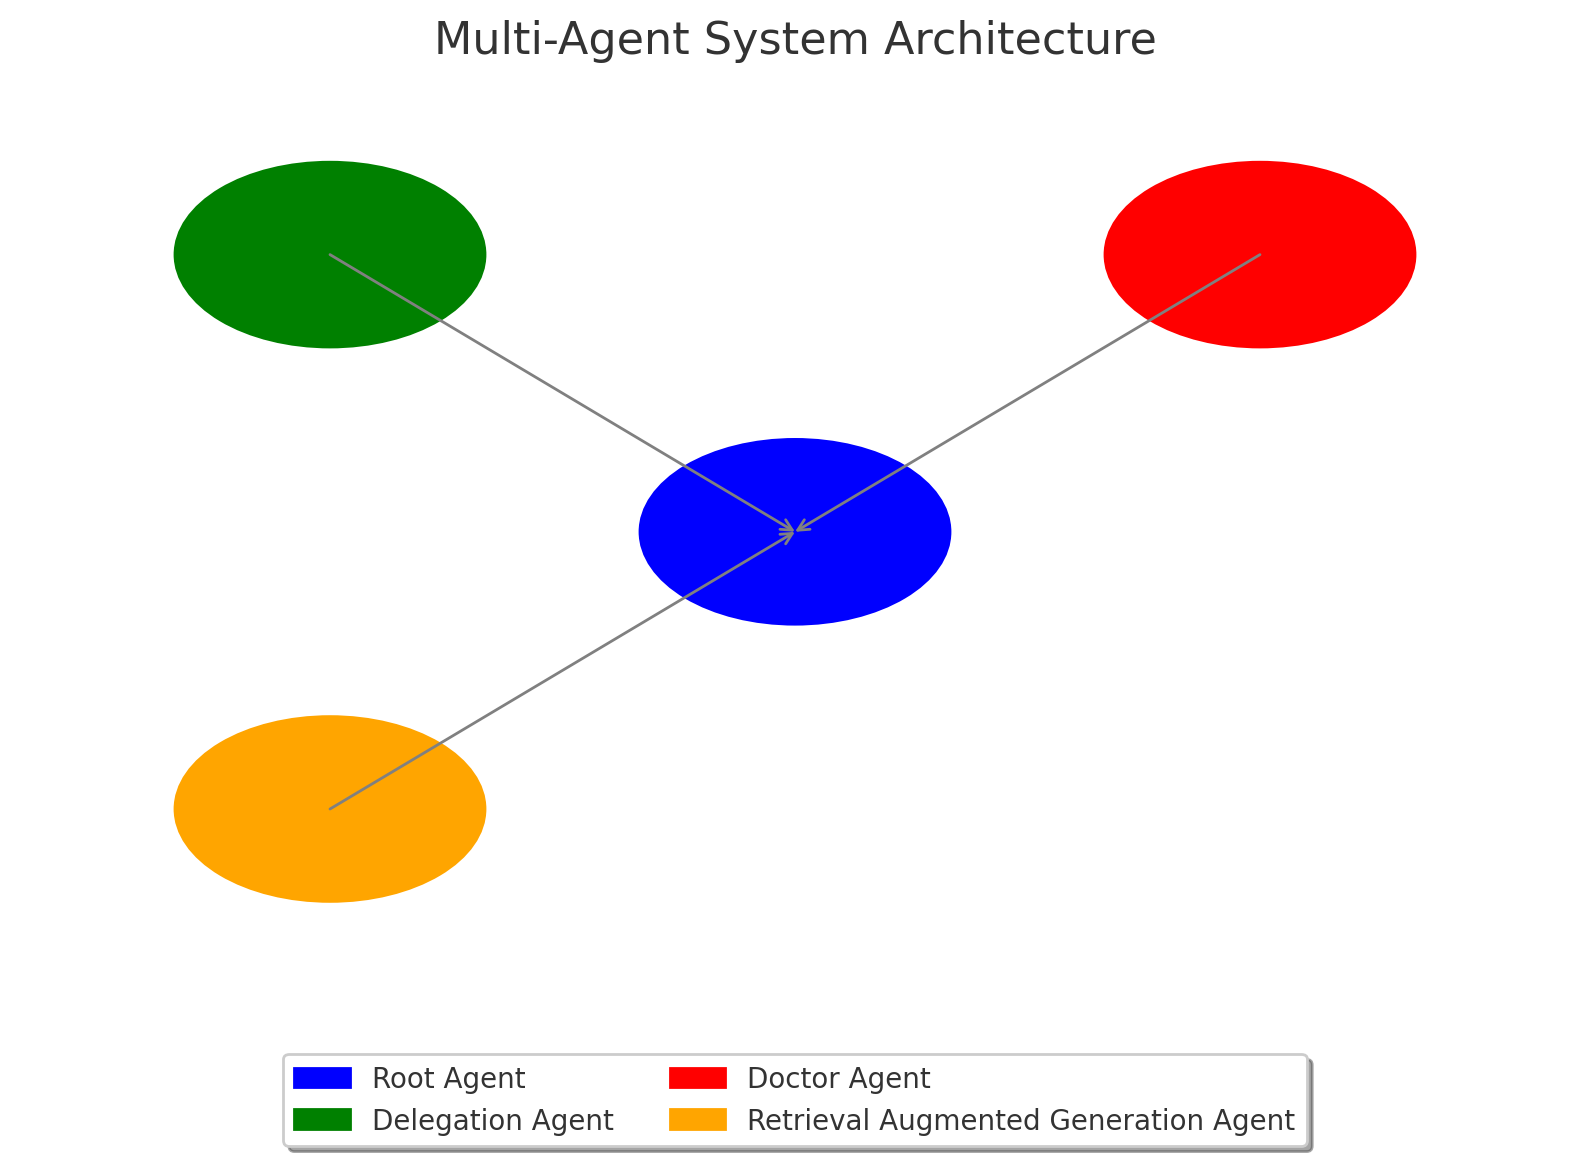
\includegraphics[scale=0.5]{60e98697-1ed7-43f9-aacd-6eb0d014d1ea.png}

Envisioning a practical scenario, one can conceptualize a hierarchical structure of agents, each tailored to fulfill specific roles within a broader system:

\begin{itemize}
	\item Root Agent: This agent embodies a general-purpose model with a foundational task of ensuring that all interactions maintain a tone of kindness and empathy. It acts as a supervisory node, overseeing the activities of subordinate agents to align them with the overarching ethical framework.
	\item Delegation Agent: Equipped with a specialized model adept in medical terminologies, this agent functions as a linguistic bridge, translating complex medical jargon into understandable language and disseminating this information to pertinent agents upon request.
	\item Doctor Agent: This agent serves as a repository of medical knowledge, encapsulating insights and feedback from healthcare professionals to enrich the system's database with expert-driven information.
	\item Retrieval Augmented Generation Agent: This agent specializes in augmenting the system's capabilities by integrating external and internal data sources, thereby enhancing the content generated in response to inputs from patients or doctors.

\end{itemize}

The architecture outlined above exemplifies the multifaceted utility of agents in orchestrating complex tasks through synergistic interactions. By facilitating seamless communication between agents, the system is not constrained by the limitations of individual models but is empowered to synthesize comprehensive outputs that encapsulate a wide array of knowledge and functionalities. This integrative approach underscores the potential of agent-based architectures to revolutionize information processing and decision-making paradigms in fields as critical as healthcare, where the precision, adaptability, and responsiveness of computational agents can significantly augment human expertise and operational efficiency.


\section{Tracing}

In the domain of computer science, tracing is a fundamental concept that facilitates the detailed examination of the execution paths of programs. This process enables developers to understand the sequential progression of code execution, from higher-level instructions to their corresponding assembly language and, eventually, the hardware-level operations. Tracing offers invaluable insights into the intricate workings of software, allowing for the identification and rectification of errors, optimization of performance, and enhancement of system reliability. In the context of healthcare applications, the ability to trace the execution of algorithms and models becomes paramount, especially when these technologies are employed to support decision-making processes in clinical settings.

The integration of tracing mechanisms within health informatics systems introduces a layer of transparency and accountability, critical for fostering trust among users, including healthcare professionals and patients. By providing a comprehensive overview of how data is processed, the basis of model-generated suggestions, and the procedural context of these recommendations, tracing empowers stakeholders with the knowledge to evaluate the efficacy and appropriateness of the computational insights offered.

The application of tracing in Kind Health systems is multifaceted, encompassing several key dimensions:

\begin{itemize}
	\item Explainability and Trust: Enhancing the clarity with which model outputs and decisions are presented, thereby facilitating better understanding and acceptance among healthcare providers and patients.
	\item Efficiency in Patient Encounters: Measuring and potentially reducing the time required for each patient interaction, thereby improving operational efficiency and patient experience.
	\item Concordance with Physician Decisions: Evaluating the degree to which model-generated recommendations align with historical physician decisions and accepted medical practices.
	\item Patient-Provider Interactions: Analyzing the frequency and quality of interactions between patients and healthcare providers within the system to optimize engagement and care delivery.
	\item Information Accuracy: Ensuring the precision and reliability of the information generated by the system, which is fundamental for clinical decision support.
	\item Diagnostic Support Accuracy: Assessing the alignment of diagnostic aids provided by the system with the professional judgments of medical practitioners, thereby augmenting the diagnostic process.
	\item Alert Identification: The system's capability to identify critical health alerts and notify healthcare providers, thereby enhancing patient safety and care responsiveness.

\end{itemize} 

The above outlined metrics will also be dynamically generated data from the conversation and the agents there are other performance related assesment that we should incroporate like cost analysis of the models and API's used. These tracing combined with agents could be automated in terms of these below outline properties that wish to build in our tech stack 


Tracing will be helpful in many cases where we can create a system threshold for the next most important component which is the key part for creatinng better output in terms of data based decsion making

\section{Evaluation Framework}

A paramount feature of any computational system, particularly within the context of healthcare informatics, is the implementation of a robust evaluation framework. This mechanism is essential for the continuous assessment and refinement of the system's performance, leveraging the extensive data repository accrued over time. The objective is to transcend conventional limitations by affording users, including healthcare professionals, the latitude to define and customize evaluation metrics tailored to their specific requirements and the nuanced dynamics of healthcare delivery.

The integration of tracing functionality serves as a foundational element in this evaluative process, offering a graphical representation of data flows and decision pathways within the system. This visualization aids in demystifying the operational intricacies of the system, thereby enabling stakeholders to engage more effectively in the evaluative process. Building upon this transparency, the proposed framework extends the capability for stakeholders to actively participate in the formulation of evaluation criteria. This participatory approach ensures that the assessment parameters are not only comprehensive but also aligned with the practical realities and exigencies of clinical practice.

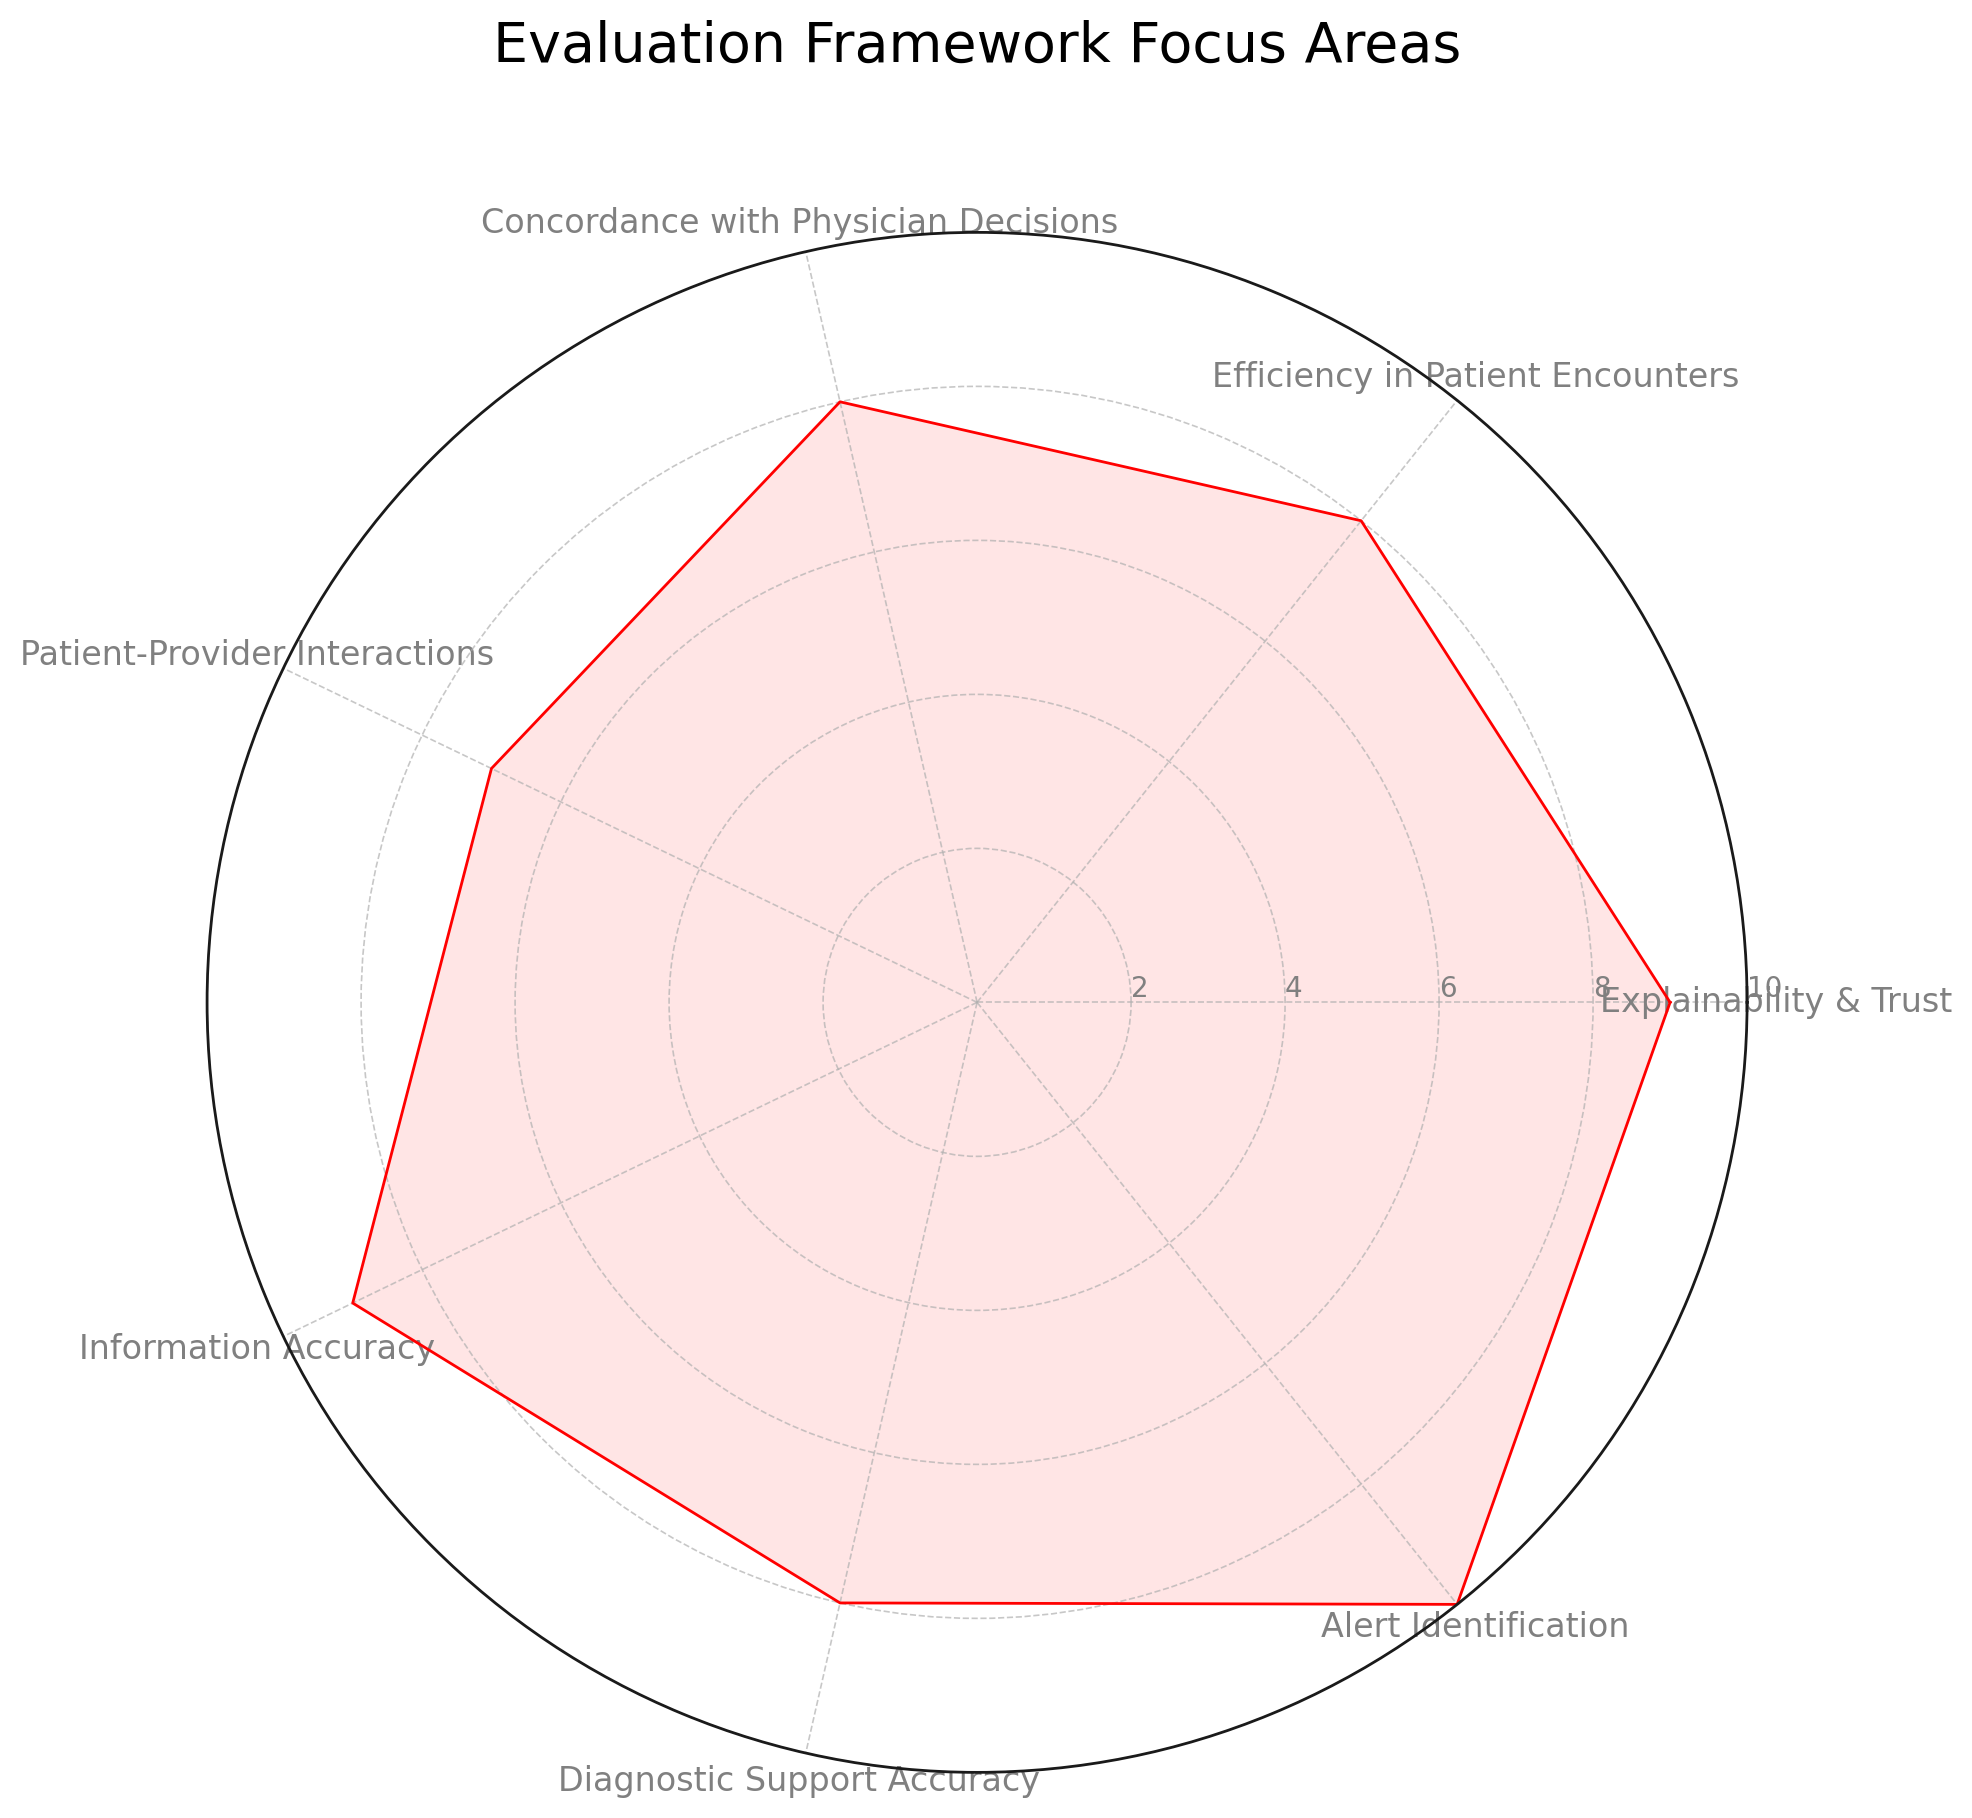
\includegraphics[scale=0.5] {0081946a-ae16-4c04-9a1a-238f2112a728.png}

Embedded within the system, these evaluation metrics function as dynamic benchmarks that guide the adaptive evolution of the system. Unlike traditional fine-tuning methodologies that primarily focus on model recalibration based on new data inputs, the envisioned approach emphasizes the application of rule-based thresholds. These thresholds act as operational parameters that can trigger system adjustments, facilitating a more nuanced and context-aware optimization process.

The practical application of this evaluative framework involves the creation of conditional scenarios, akin to test cases, which enable the systematic examination of system outputs against predefined standards. This methodology allows for the generation of actionable insights, quantified through specific metrics, which can inform strategic modifications to the system. The ultimate aim is to enhance the system's efficacy by eliminating data anomalies, reducing bias, and augmenting the contextual relevance of its outputs.

To expedite the development of this sophisticated evaluation mechanism, it is prudent to leverage existing implementations within the domain. By adapting and integrating proven methodologies, the development process can be streamlined, thereby accelerating the enhancement of the system's evaluative capabilities. This approach not only ensures the technical robustness of the evaluation framework but also facilitates its alignment with the evolving needs of healthcare practitioners and patients, thereby contributing to the overarching goal of improving healthcare outcomes through advanced computational tools.

Different type of evaluative parameters that we will implement.
\begin{itemize}
	\item G Eval
	\item Summaration
	\item Answer relevancy 
	\item contextual reasoning
	\item Bias 
	\item Toxicity
	\item Medical Readiness
\end{itemize}

\section{Conclusion}

Throughout this discourse, we have explored various facets of our system, emphasizing its core functionalities and operational principles. However, it is pertinent to acknowledge that certain ancillary yet crucial aspects have not been extensively discussed. Notably, our implementation strategy is underpinned by the principles of modularity, reusability, and loose coupling. These foundational tenets are instrumental in fostering a flexible and scalable system architecture, conducive to iterative enhancements and adaptability to evolving technological landscapes.

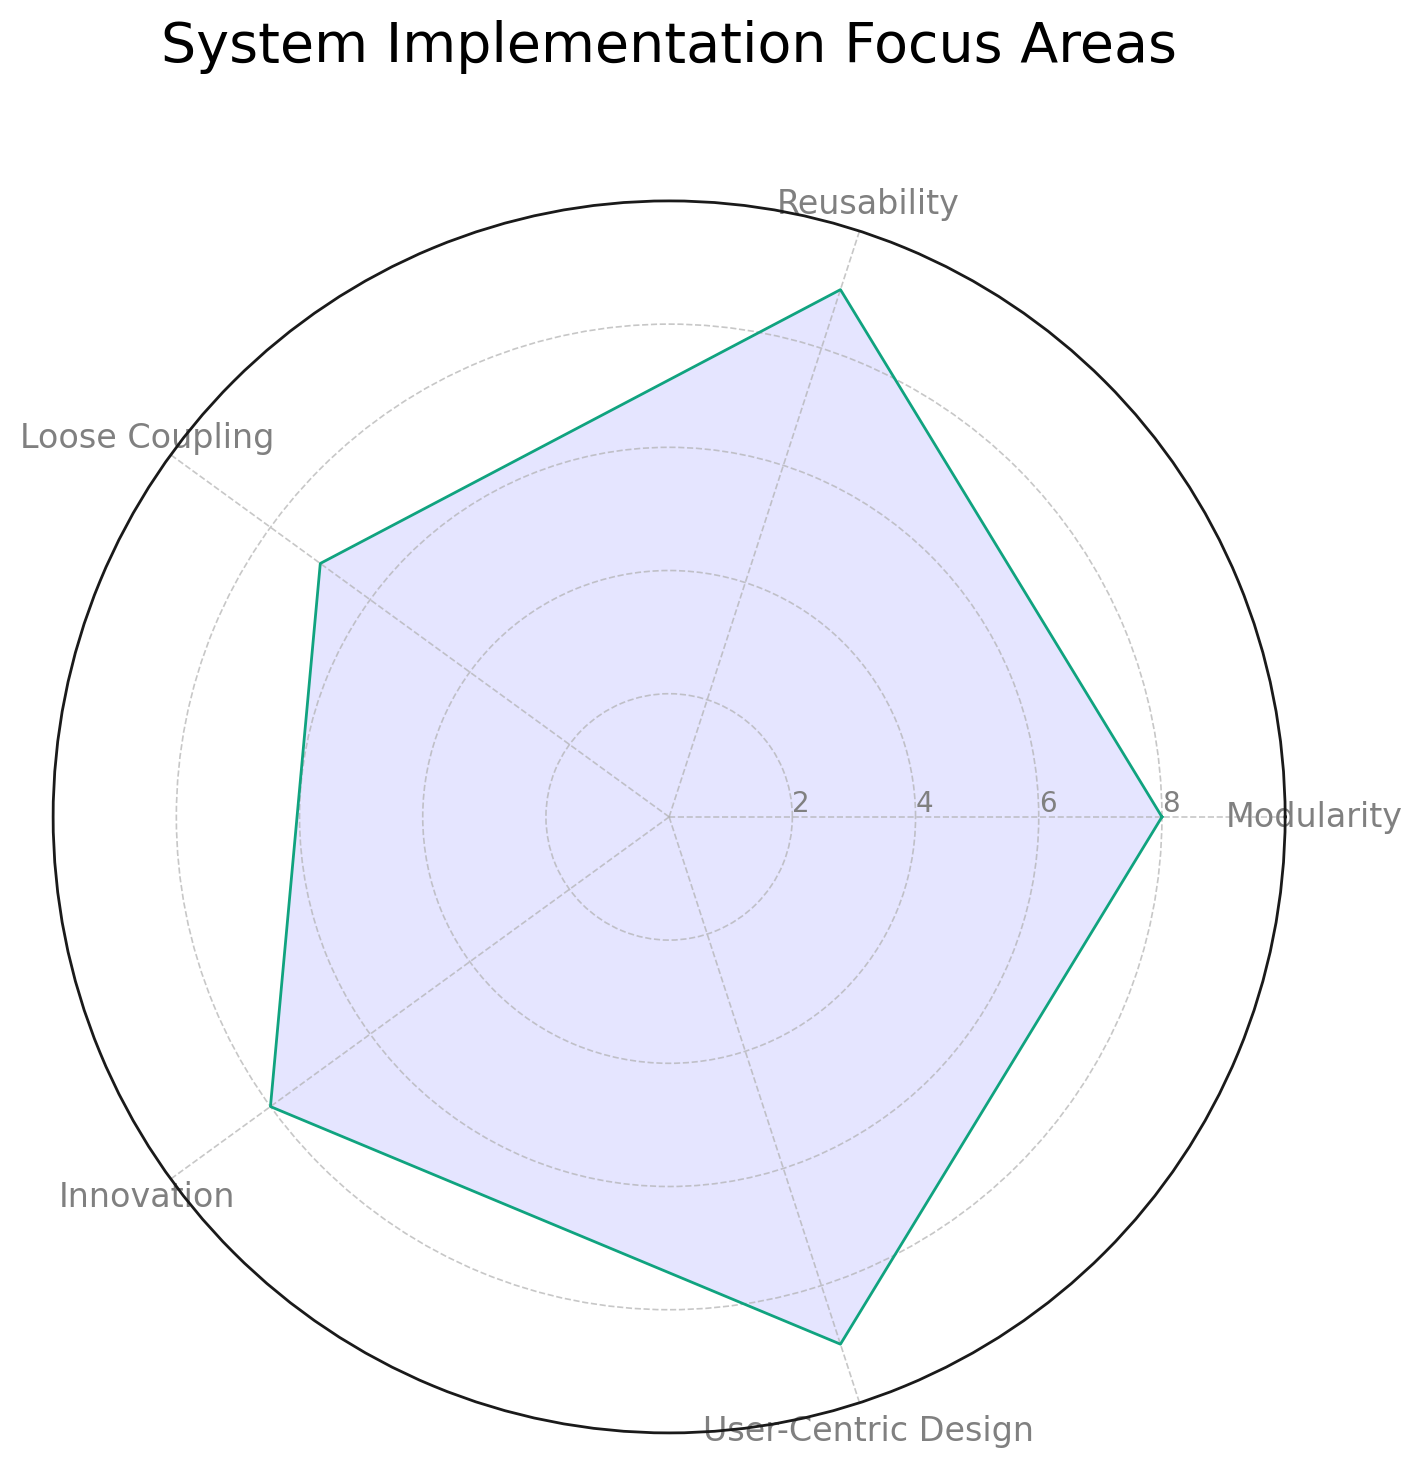
\includegraphics[scale=0.5]{f789fce4-69a3-4e83-aec2-e23580880be8.png}


In alignment with our strategic focus, we have adopted an approach that, while not entirely unprecedented, is characterized by a degree of innovation in its application. This involves a carefully curated technological stack designed to harmonize with our system's architectural requirements. Specifically, we plan to utilize the Langroid framework, renowned for its efficacy in facilitating multi-agent system configurations. This choice is predicated on Langroid's compatibility with our system's design ethos, particularly its emphasis on modularity and agent autonomy.

Furthermore, we intend to leverage the Deep Eval SDK as a cornerstone for developing our evaluation framework. The SDK's capabilities will be instrumental in enabling the dynamic definition and application of evaluation metrics, thereby enhancing the system's responsiveness to user feedback and evolving operational contexts.

Complementing these components, we propose the development of a bespoke tracing mechanism, accompanied by a user interface (UI) that synergistically integrates the system's diverse functionalities. This interface will not only serve as a conduit for user interaction but also as a visual representation platform, elucidating the complex data flows and decision-making processes inherent in the system's operation.

The confluence of these technological choices and design principles underscores our commitment to creating a system that is not only robust and efficient but also aligned with the best practices of software engineering. This holistic approach ensures that the system remains at the forefront of innovation, providing a scalable and user-centric solution to the challenges faced in its intended domain of application.

\bibliographystyle{plainnat}
\bibliography{references}

\end{document}
